%\section{Research Objectives}

%The desired outcome of this PhD thesis is to improve the \gls{fMRI} and the \gls{DMI} at 9.4 T using \gls{bSSFP} acquisition to study the human brain. In the first publication (see \cref{sec:paper1})  

%\begin{itemize}
%	\item cartesian bSSFP has more or less fixed TE/TR parameter space
%	\end{itemize}


\section{Summary}

We have demonstrated two applications of \gls{bSSFP} acquisition to investigate brain function at 9.4 T.
In Publication 1, the encoding efficiency of passband-bSSFP was improved using a 3D stack-of-spirals acquisition combined with parallel imaging at a challenging ultra-high field strength, thereby improving the practicality of bSSFP-BOLD to a level comparable with popular \gls{GRE}-\gls{EPI}. This work was aimed to advance the development of an fMRI technique with reduced sensitivity to macro-vascular biases and geometric distortions suitable for high-fields. To improve image quality, we incorporated a slice-selective binomial pulse for fat suppression and a reconstruction model that accounts for system imperfections such as trajectory deviations and spatial $B_0$ inhomogeneity. We further explored the acquisition parameters (e.g., TR and TE) space afforded by the non-Cartesian bSSFP sequence and proposed optimal protocols to maximize functional sensitivity. Functional activation maps obtained from both high-resolution thin-slab (0.6 mm and 0.8 mm isotropic) and whole-brain (1.2 mm isotropic) experiments exhibited localized activation without geometric distortion. 

In publication 2, we developed \gls{bSSFP} acquisition techniques and novel processing methods to enhance the sensitivity of \gls{DMI}. The favorable $T_2/T_1$ of deuterated metabolites yielded a much higher SNR improvement with \gls{bSSFP} compared to spoiled \gls{GRE} sequences. Two encoding variants \gls{CSI} and multi-echo of \gls{bSSFP} acquisition were tested with phantom measurements and subject measurements with oral [6,6'-$^2H_2$]-glucose intake. Due to the significant spatial $B_0$ inhomogeneity in the human head at 9.4 T, phase-cycling was employed to reduce the off-resonance sensitivity, albeit with a moderate reduction in \gls{SNR}. Furthermore, we showed the phase-cycling provides additional spectral encoding which can provide flexibility to reduce the \gls{TR}, thereby potentially increasing off-resonance insensitivity even further. A notable observation was that the reference method, based on the vendor's 3D \gls{CSI} implementation, utilized optimal protocols for efficient averaging and SNR-performant \gls{FISP}/\gls{SSFP}-\gls{FID} acquisition with no RF spoiling. That combined with the SNR loss of phase-cycling, the achieved SNR enhancement of up to 25\% is much lower the reported numbers in preclinical studies where they used RF-spoiled FLASH acquisition. The desirable \gls{PSF} of acquisition-weighting used in \gls{CSI} variant showed a better SNR performance than the uniform k-space weighting of multi-echo \gls{bSSFP} variant. The flexibility of the proposed IDEAL-modes algorithm greatly simplifies the processing of phase-cycled spectroscopic bSSFP data and produces reliable metabolite maps without the explicit knowledge of the spatial off-resonance map , flip angle map, and relaxation times of the deuterium metabolites. The spectral resolution was sufficient to reliably separate the glucose uptake and downstream metabolites in the brain.   



\section{Outlook}

Passband-bSSFP offers a promising alternative to traditional GRE-BOLD fMRI at high field, leveraging vessel size specificity to isolate BOLD signals originating near small vessels such as capillaries to be closer to neuronal activity and to minimize contributions from larger vessels.  In publication 1, we addressed a key practical limitation, the slow acquisition speed, with efficient spiral acquisition. However, in vivo validation of the vessel size specificity is crucial for its broader adoption. While demonstrated in simulations\cite{baez-yanezImpactVesselSize2017} and phantom experiments with micro-spheres \cite{schefflerBOLDSensitivityRapid2019}, replicating these findings in vivo remains challenging. In a recent study, the superior signal stability of bSSFP across cortical layer compared with GRE-BOLD was demonstrated with resting-state data . To explore along these lines, we conducted some experiments to investigate the evidence of vessel specificity of bSSFP-BOLD contrast.

\subsection{Investigating large vessels bias}
In this preliminary study, the BOLD signal changes were investigated near large vessels segmented from a co-registered high-resolution Cartesian \gls{GRE} scan. The underlying hypothesis is that bSSFP-BOLD should exhibit lower signal changes near large veins compared to GE-BOLD, reflecting improved spatial specificity. As shown in \cref{fig:vesselDistance}, the bSSFP BOLD signal changes near large vessels demonstrates marginally reduced signal changes, suggesting a degree of vessel specificity. This effect becomes more pronounced in the bSSFP functional experiment conducted with a shorter TR and higher spatial resolution, where the suppression of large-vessel contributions is more clearly visible.

\begin{figure}[H]
	\centering
	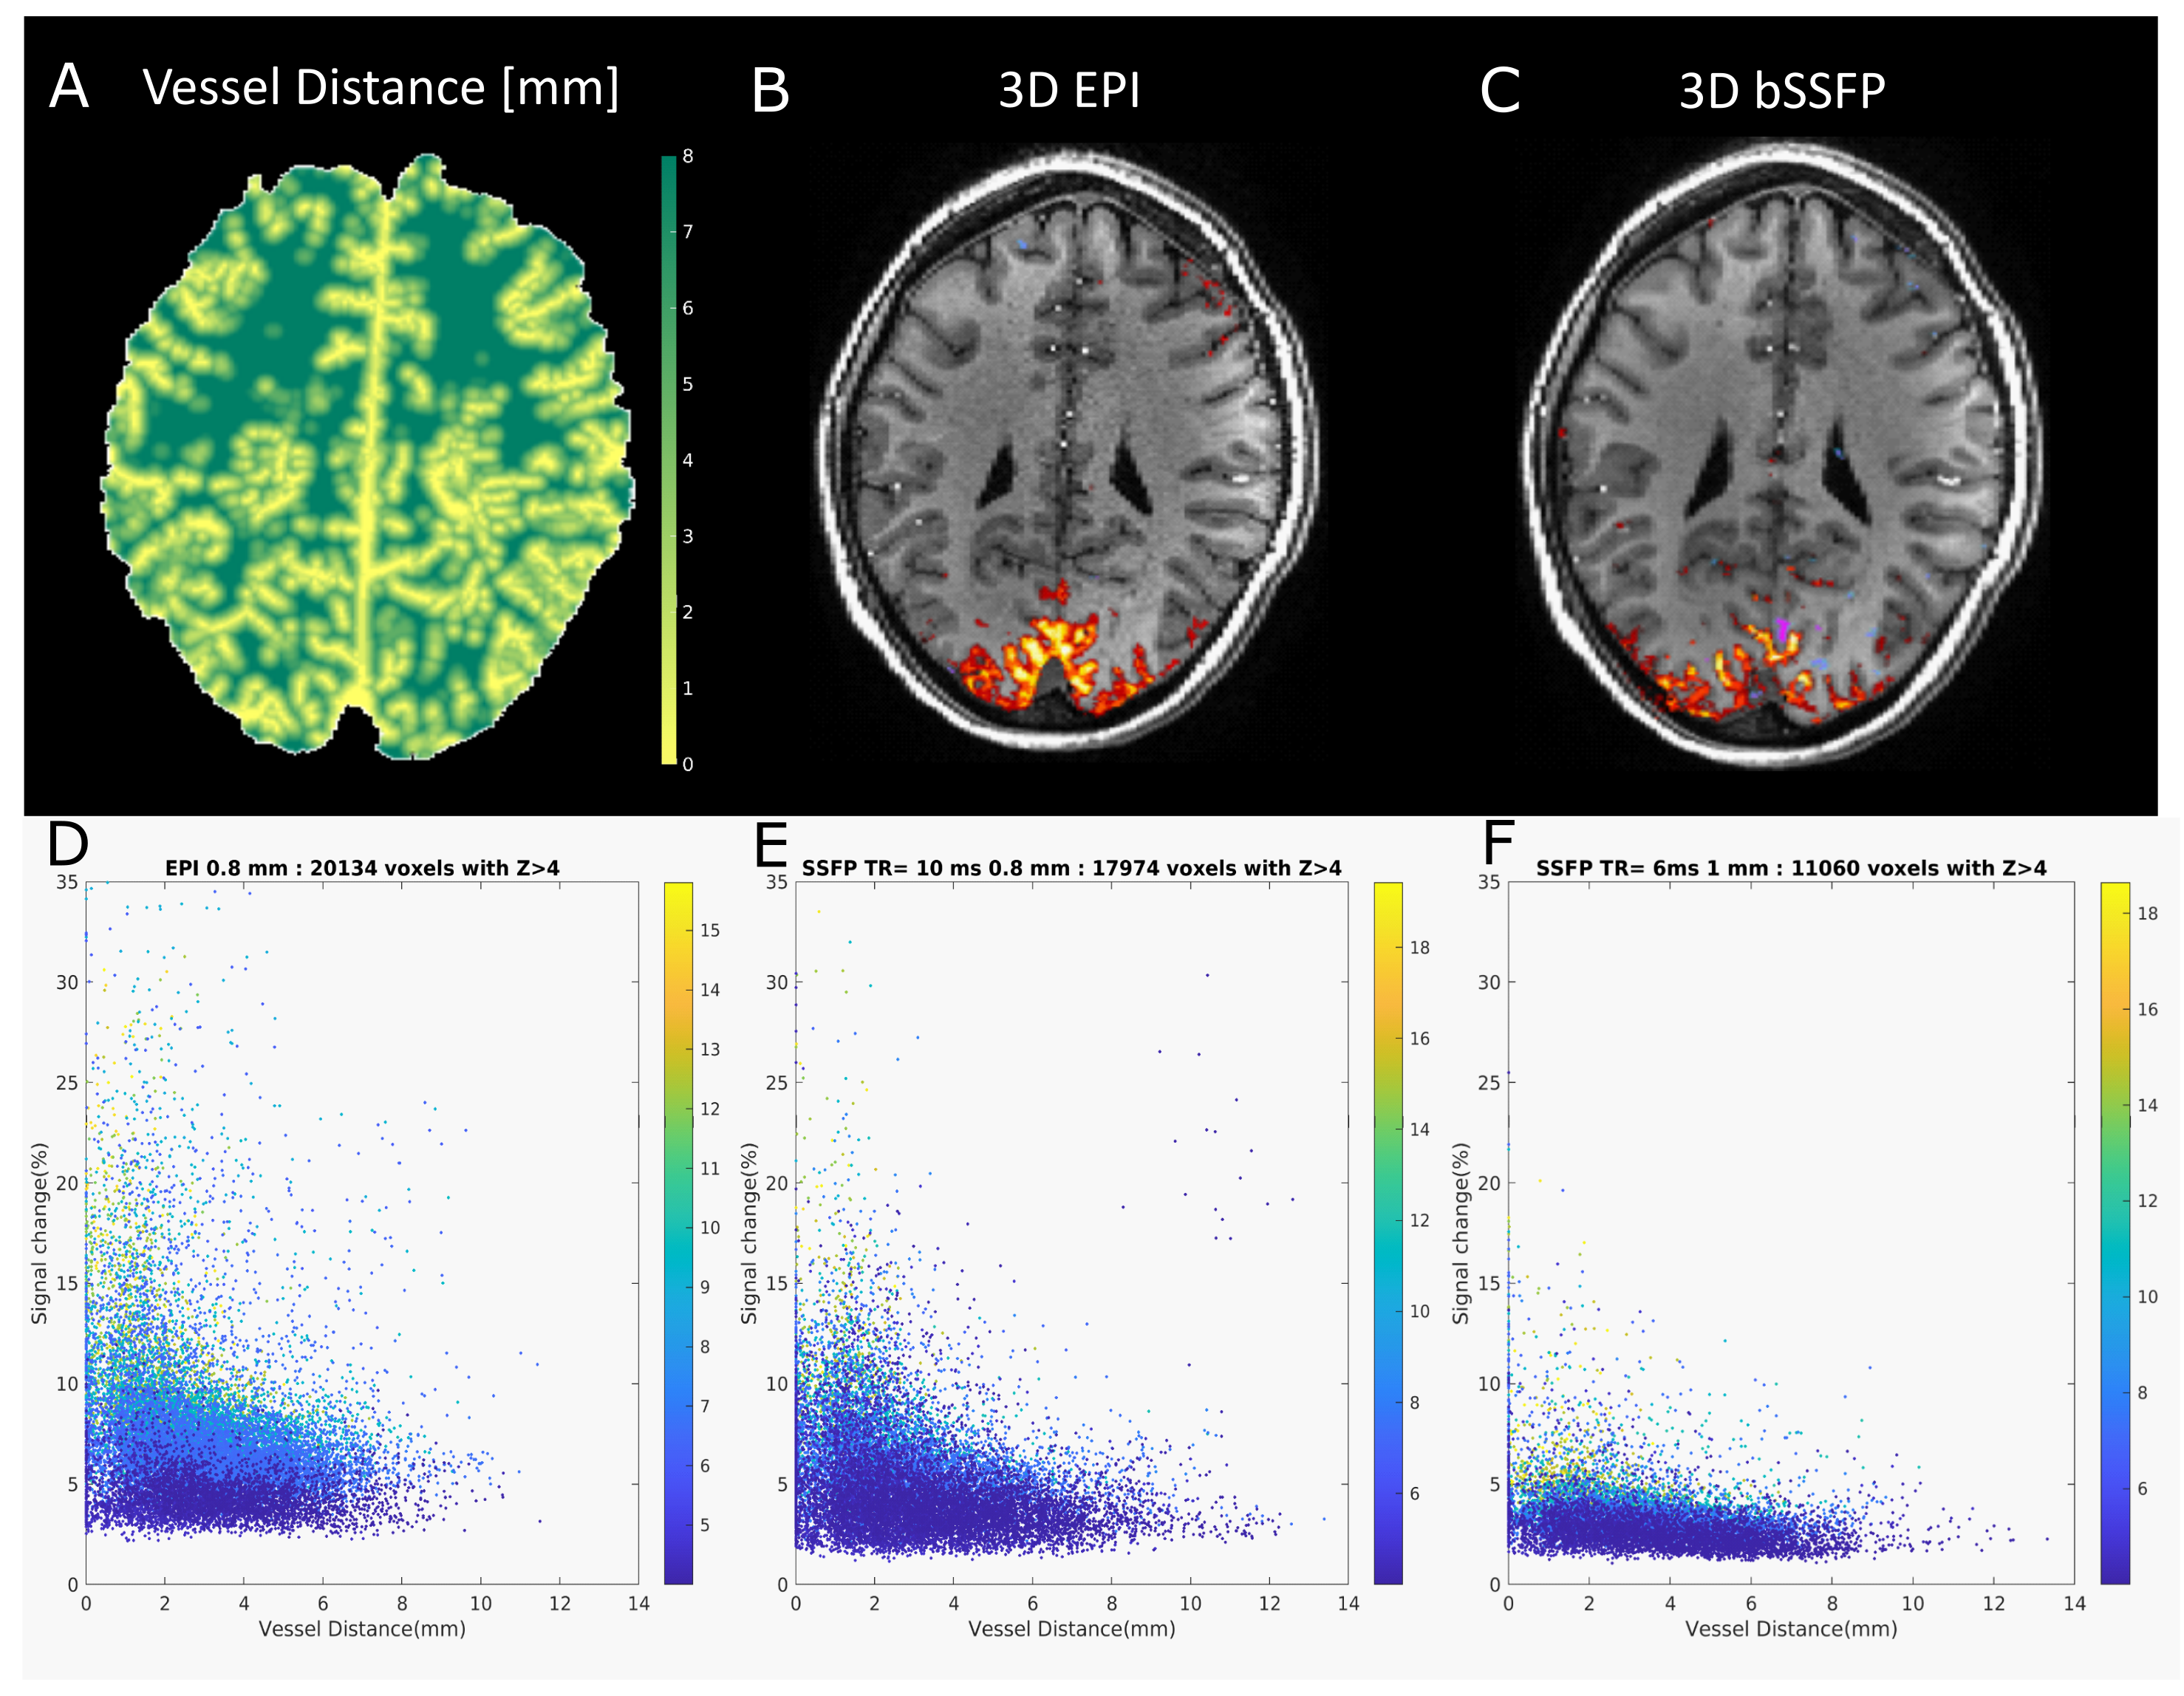
\includegraphics[width=1.0\textwidth]{graphics/vesselDist.png}
	\caption{The dependency of vessel distance and signal change for GE-EPI and bSSFP acquisition. A) vessel distance in mm from large veins segmented by Frangi filter on a high resolution Cartesian GE-scan (TE=16 ms, 0.4 mm isotropic resolution). Exemplary anatomical axial image with GE-EPI (0.8 mm isotropic resolution) and spiral-bSSFP activation map (0.8 mm isotropic resolution). The corresponding signal change in the significantly activated voxels from the activation maps B and C are plotted against the vessel distance in D and E respectively. F) A similar plot is shown for bSSFP functional experiment with TR=6ms and 1mm isotropic voxels.}
	\label{fig:vesselDistance}
\end{figure}


\subsection{BOLD signal change in refocusing modes}
With the complicated vasculature in the human brain, demonstrating small vessel specificity of the bSSFP-BOLD is challenging. An alternative approach would be to show the BOLD signal change in the refocusing echo pathways in bSSFP-BOLD to show its spin-echo behavior. In the preliminary investigation\cite{iyyappanvalsalaInvestigationBSSFPFrequency2024},

\begin{figure}[H]
	\centering
	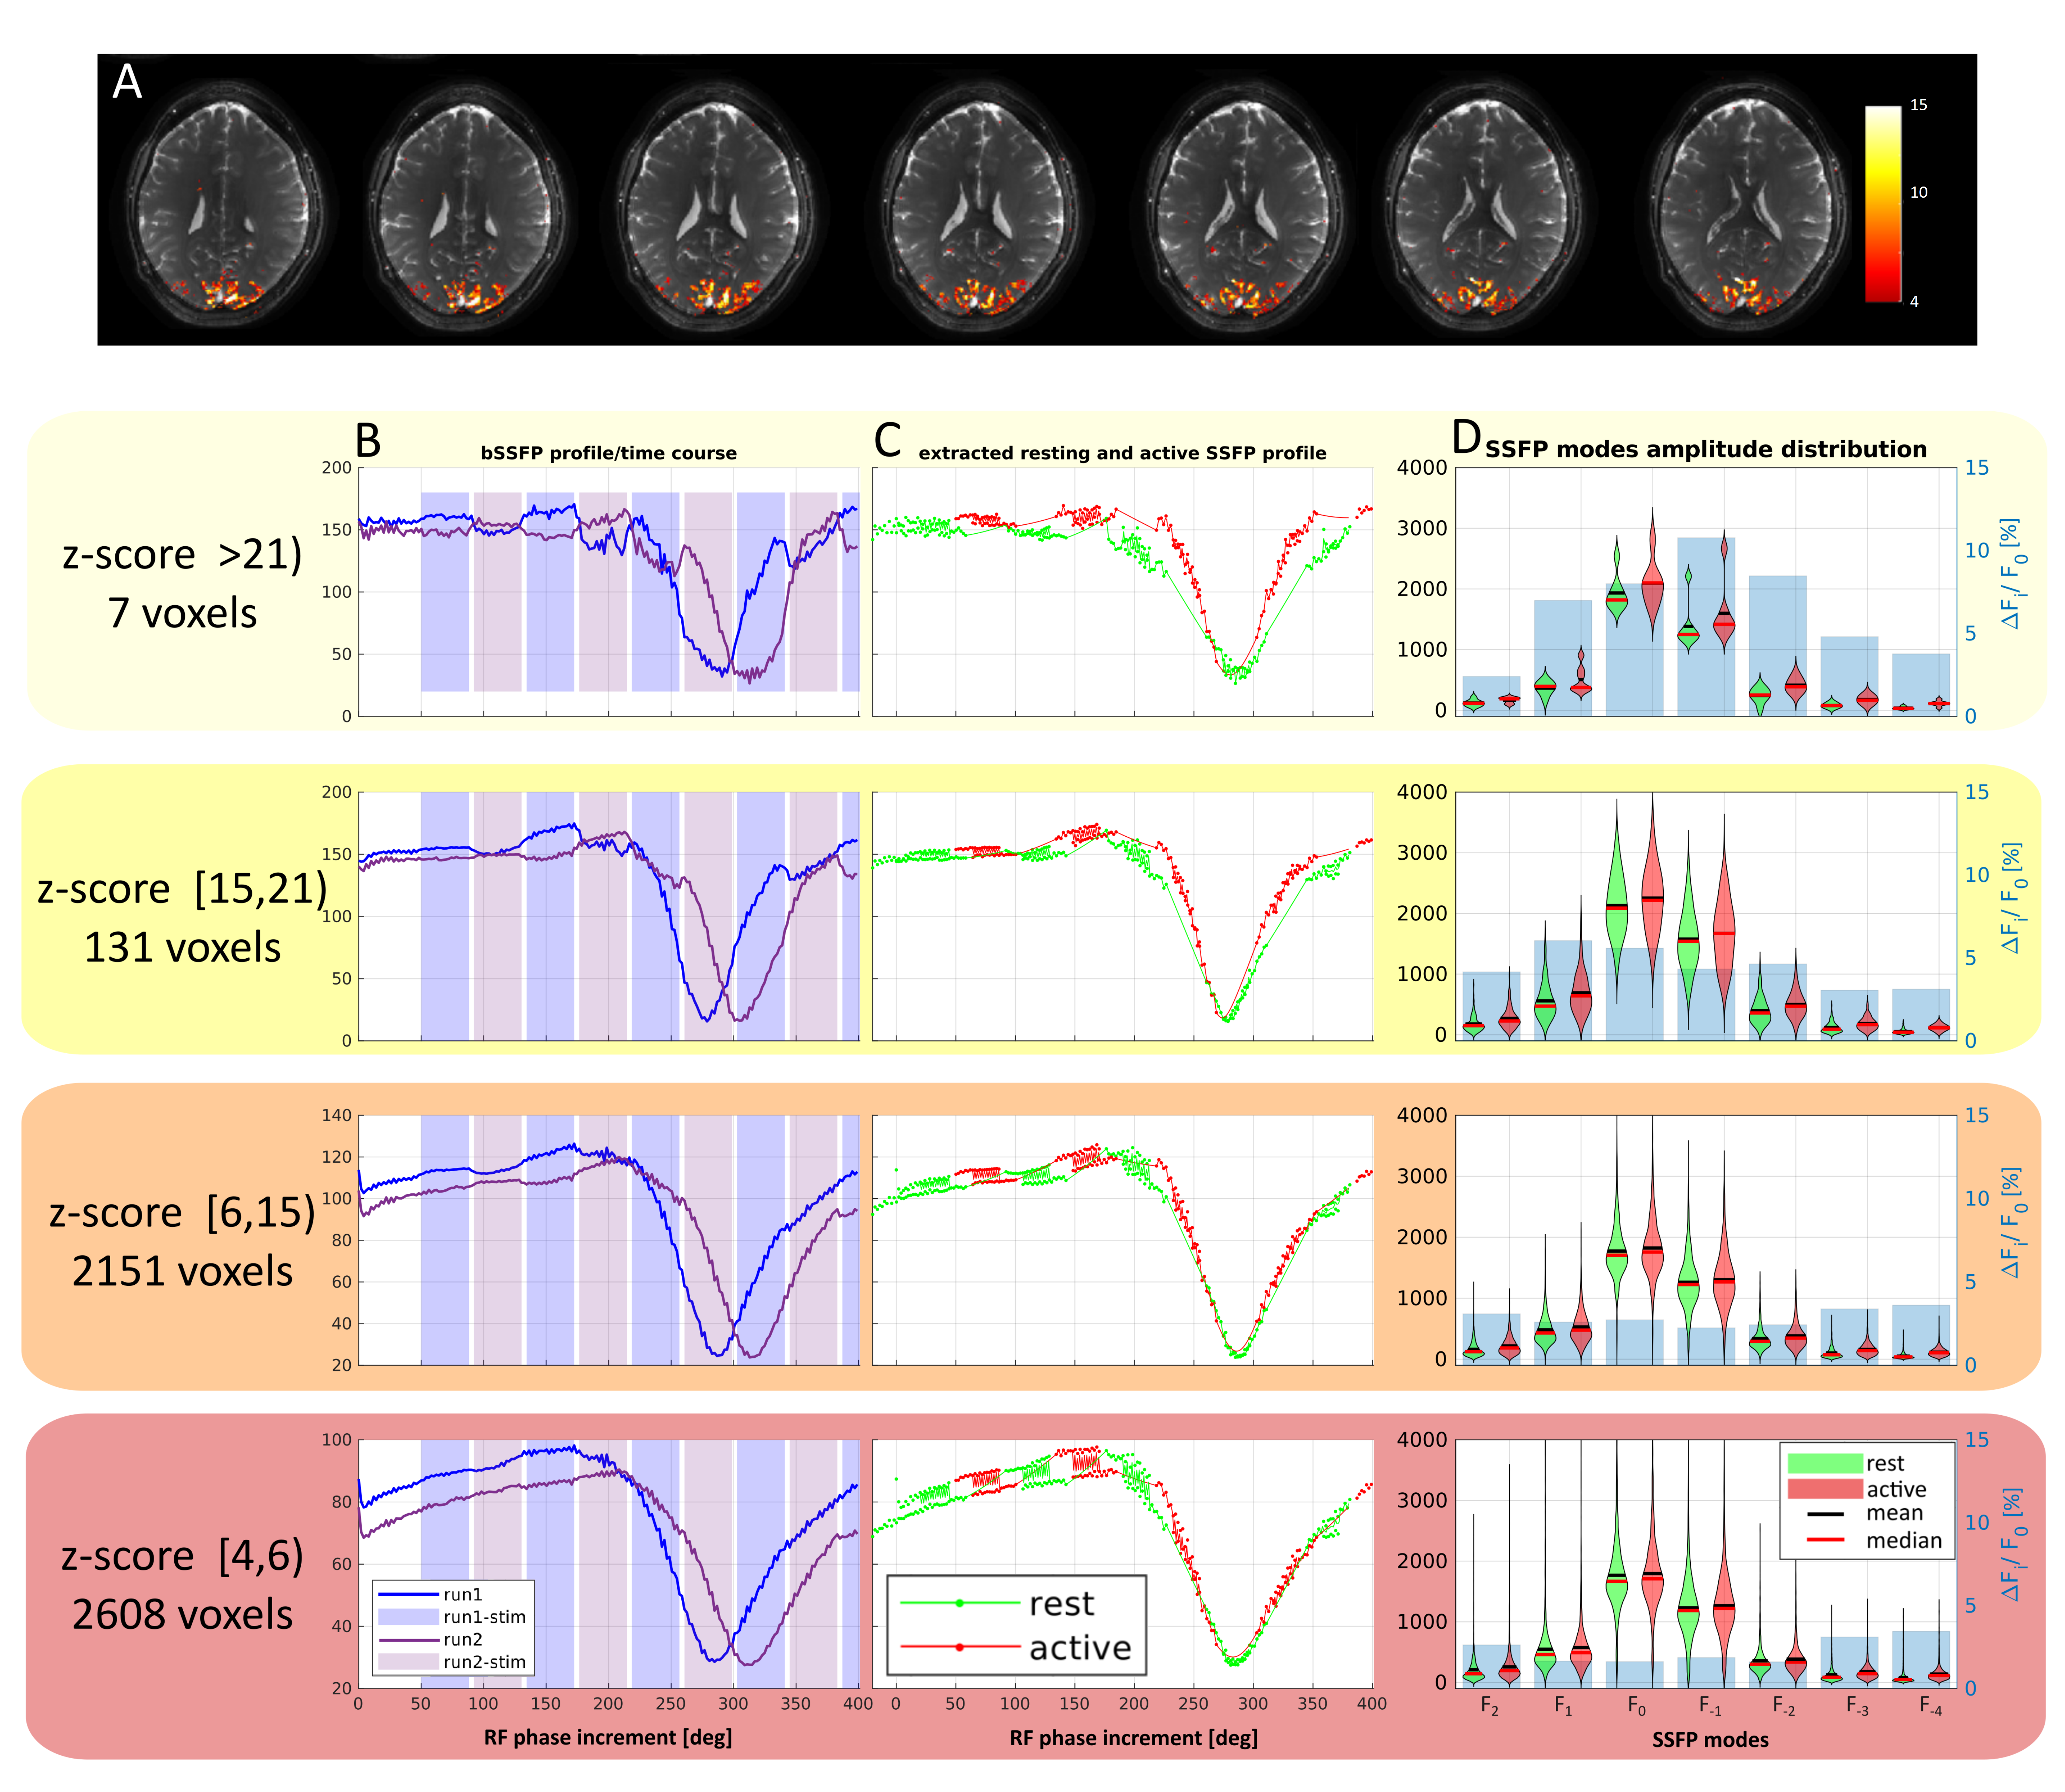
\includegraphics[width=1.05\textwidth]{graphics/bSSFPBOLD_modes.png}
	\caption{bSSFP frequency response during a functional experiment. A) The activation maps from a passband experiment (TR= 10 ms) used for selecting the activated voxels. The average time courses from the functional experiments with phase cycling [B], the extracted  average bSSFP profiles during resting and active conditions [C] and the SSFP mode amplitude distribution during resting and active conditions D of all voxels with z-scores>21. Similarly, the activated voxels with lower z-scores are shown below.}
	\label{fig:bssfpBOLDmodes}
\end{figure}


\subsection{Transient bSSFP-BOLD}

Another interesting observation made possible because of the acquisition speed of 3D spiral-bSSFP sequence is the the bSSFP-BOLD contrast inversion during the transient phase. The use of 2D multi-slice \gls{bSSFP} sequence to improve coverage in passband \gls{fMRI} studies\cite{reynaudMultislicePassbandBSSFP2019b,blazquezfrechesBOLDfMRIMouseAuditory2018} could result in measuring bSSFP-BOLD contrast in the transient state. Rahel et al.\cite{heuleInvertedBOLDSignal2024} show that the bSSFP-BOLD contrast evolve along the pulse train. Particularly, the contrast is inverted for large vessels during the early transient phase as shown in \ref{fig:negBOLD}. However, the effect could not be observed \textit{in vivo} with conventional Cartesian encoding even with a segmented approach\cite{heuleInvertedBOLDSignal2024}. With the acceleration of spiral encoding and parallel imaging, it is possible to acquire whole brain volume within 50 excitations. Thereby enabling the sampling of early transient phase of bSSFP-BOLD contrast. For the checkerboard stimulus, most of the activated voxels with positive correlation during the passband experiment show negative correlation to the stimulus paradigm in the transient bSSFP-BOLD.    

\begin{figure}[H]
	\centering
	
\includegraphics[width=0.8\textwidth]{graphics/negBOLD.png}
	\caption{Inverted BOLD signal changes in the transient phase of passband balanced SSFP. A) BOLD-related signal changes simulated by a Monte Carlo approach in units of the equilibrium magnetization $M_0$\cite{heuleInvertedBOLDSignal2024}. The Activation maps reference from passband-bSSFP and transition-band functional experiment are overlaid on anatomical reference in panels B and C, respectively. In both cases, whole brain functional volume was acquired in ~300 ms with 2.5 mm isotropic nominal resolution. During transition-band experiment, the recovery time between volumes was 4 s, increasing the volume TR to 4.3 s. Other imaging parameters: TR=6.1 ms,TE=0.69 ms,FA= $15^\circ$ and parallel imaging factor= 4x2.}
	\label{fig:negBOLD}
\end{figure}


- discuss about un-balanced fmri papers
- simulations
- SE - occular dominence column
- paradigm design

\subsection{concurrent monitoring}


\begin{figure}[H]
	\centering
	\includegraphics[width=1.0\textwidth]{graphics/concurrentmonitoring.png}
	\caption{Concurrent trajectory monitoring with the field-probe insert for a 16Tx/32Rx coil. (A)shows the individual layers of the coil assembly from the inside to the outside. A 2D 0.75 mm multi-shot spiral (7 ms readout) acquisition is reconstructed with nominal trajectory (B),  trajectory from gradient impulse response function (GIRF) predictions (C) , measured trajectory (D), measured trajectory with B0 correction (E) and parallel imaging (F). The second row shows the image differences to highlight the improvements (G-I,K) and field map (J) used for B0 correction. }
	\label{fig:concurrentmonitoring}
\end{figure}


Other still open problem.
- real time spiral reconstruction
- motion
- intershot phase correction
- flow effects: Significant signal changes in BOLD-fMRI arise due to the inflow of the fresh spins flowing into the imaging volume. Eventhough inflow effects is minimized with 3D imaging with thick slabs and low flip angle, inflow effects must be investigated further.

